% !TEX encoding = UTF-8 Unicode
\chapter{Architektur}
\label{kapitel_architektur}
Die nachfolgende Abbildung zeigt die Architektur von Esper.
Dabei ist sie, für einen einfacheren Einstieg in Esper, auf die wichtigsten Komponenten beschränkt.

\begin{figure}[ht]
	\centering
	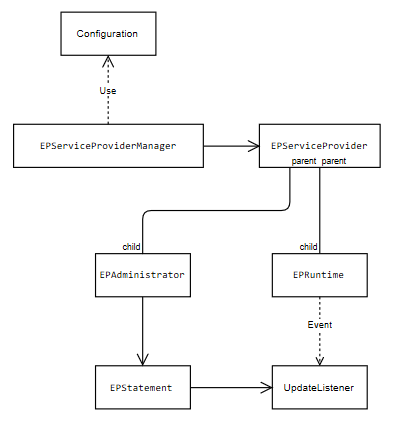
\includegraphics{images/Architektur.png}
	\caption{Architektur von Esper}
	\label{architektur}
\end{figure}

Die \textbf{Configuration}-Klasse wird verwendet, um die Esper-Engine zu konfigurieren. Unter anderem lassen sich dort die Event-Typen registrieren, die verarbeitet werden sollen. Neben den Event-Typen, können Plugins registriert werden. Durch Plugins werden benutzerdefinierte Funktionen eingebunden (z.B für den Vergleich von Geo-Koordinaten).
Nachfolgend zeigt die Basis-Konfiguration, für das Szenario, dieser Ausarbeitung:

\begin{lstlisting}[caption={Basis-Konfiguration}\label{lst:basisKonfiguration},captionpos=t,language=JAVA]

import com.espertech.esper.client.Configuration
import de.htwg.da.esper.sample.event.GameActionEvent;
import de.htwg.da.esper.sample.event.GameEndEvent;
import de.htwg.da.esper.sample.event.GameStartEvent;

Configuration config = new Configuration();

// Register event types to observe
config.addEventType("GameStart",GameStartEvent.class.getName());
config.addEventType("Action", GameActionEvent.class.getName());
config.addEventType("GameEnd", GameEndEvent.class.getName());
\end{lstlisting}

In der Beispiel-Konfiguration werden die Event-Typen GameStartEvent, GameActionEvent und GameEndEvent registriert. Plugins werden nicht verwendet.

Über die \textbf{EPServiceProviderManager}-Klasse kann der \textbf{EPServiceProvider} erhalten werden:
 
\begin{lstlisting}[caption={EPServiceProvider}\label{lst:epServiceProvider},captionpos=t,language=JAVA]

import com.espertech.esper.client.*;

EPServiceProvider cep = EPServiceProviderManager.
				getProvider("MyEsperProvider", config);
\end{lstlisting}
 
 
Der erste Parameter stellt eine eindeutige Bezeichnung für den Provider dar. Dadurch ist es möglich, mehrere \textbf{EPServiceProvider} und damit mehr als eine Esper-Engine parallel zu verwenden. Als zweiter Parameter wird die zuvor  erstellte Konfiguration (siehe Quelltext \ref{lst:basisKonfiguration}) verwendet.

Der \textbf{EPServiceProvider} hält die Referenzen auf die Klassen \textbf{EPAdministrator} und \textbf{EPRuntime}. 